\begin{sol}[1](Résolu par Matthias Schuller)

On a $3^{2n}=9^n$,
or $9 \equiv 2 [7]$,
donc pour tout $n \in \mathbb{N}$, $9^n \equiv 2^n [7]$,
donc $3^{2n}-2^n \equiv 0 [7]$.

\end{sol}

\begin{sol}[5](R\'esolu par Lo\"ic Chevalier)
Il y a 32 grains au maximum car il y a au plus 4 grains par ligne sur 8 lignes. Voici un exemple de distribution \`a 32 grains :

\[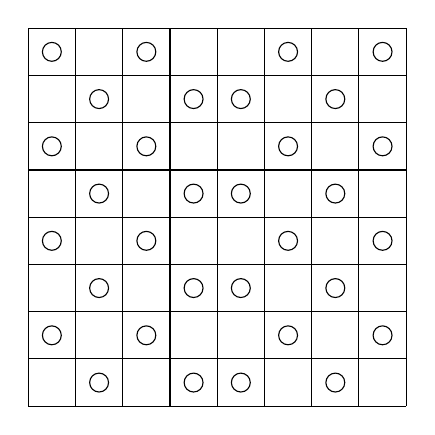
\begin{tikzpicture}[scale=0.3]
\draw (0, 0)--(0,16);
\draw (2, 0)--(2,16);
\draw (4, 0)--(4,16);
\draw (6, 0)--(6,16);
\draw (8, 0)--(8,16);
\draw (10, 0)--(10,16);
\draw (12, 0)--(12,16);
\draw (14, 0)--(14,16);
\draw (16, 0)--(16,16);

\draw (0,0)--(16,0);
\draw (0,2)--(16,2);
\draw (0,4)--(16,4);
\draw (0,6)--(16,6);
\draw (0,8)--(16,8);
\draw (0,10)--(16,10);
\draw (0,12)--(16,12);
\draw (0,14)--(16,14);
\draw (0,16)--(16,16);

\draw (1,15) circle (0.4);
\draw (1,11) circle (0.4);
\draw (1,7) circle (0.4);
\draw (1,3) circle (0.4);
\draw (3,13) circle (0.4);
\draw (3,9) circle (0.4);
\draw (3,5) circle (0.4);
\draw (3,1) circle (0.4);

\draw (5,15) circle (0.4);
\draw (5,11) circle (0.4);
\draw (5,7) circle (0.4);
\draw (5,3) circle (0.4);
\draw (7,13) circle (0.4);
\draw (7,9) circle (0.4);
\draw (7,5) circle (0.4);
\draw (7,1) circle (0.4);


\draw (11,15) circle (0.4);
\draw (11,11) circle (0.4);
\draw (11,7) circle (0.4);
\draw (11,3) circle (0.4);
\draw (9,13) circle (0.4);
\draw (9,9) circle (0.4);
\draw (9,5) circle (0.4);
\draw (9,1) circle (0.4);

\draw (15,15) circle (0.4);
\draw (15,11) circle (0.4);
\draw (15,7) circle (0.4);
\draw (15,3) circle (0.4);
\draw (13,13) circle (0.4);
\draw (13,9) circle (0.4);
\draw (13,5) circle (0.4);
\draw (13,1) circle (0.4);


\end{tikzpicture}\]
\end{sol}

\begin{sol}[22](R\'esolu par Matthias Schuller)
Le nombre $\frac{a^{2b+1}b-1}{a+1}$ doit \^etre un entier, donc $a+1$ divise $a^{2b+1}b-1$. On a donc que $a+1$ divise
\[(a^{2b+1}b-1)+(a+1)=a(a^{2b}b+1).\]
Or $a+1$ n'a aucun diviseur en commun avec $a$ car leur diff\'erence est 1, donc $a+1$ divise $a^{2b}b+1$ et donc aussi
\[(a^{2b}b+1)-(a+1)=a(a^{2b-1}b-1).\]
Par le m\^eme argument, on trouve que $a+1$ divise $a^{2b-1}b-1$. On se retrouve alors avec la formule du d\'ebut, mais avec l'exposant de $a$ diminu\'e de 2. En particulier on retrouve toujours un exposant impair. On peut alors refaire le m\^eme argument jusqu'\`a ce que l'exposant de $a$ soit \'egal \`a 1. On trouve alors que $a+1$ divise $ab-1$ et donc aussi
\[(ab-1)+(a+1)=a(b+1),\]
et donc $a+1$ doit diviser $b+1$.\\

Avec l'autre entier $\frac{b^aa+1}{b-1}$ on trouve que $b-1$ divise $b^aa+1$. On a donc que $b-1$ divise
\[(b^aa+1)+(b-1)=b(b^{a-1}a+1).\]
Toujours par le m\^eme argument, on obtient que $b-1$ divise $b^{a-1}a+1$ (noter que $b-1$ peut diviser $b$ si $b=2$, mais alors $b-1$ divise tout nombre). On se retrouve alors avec la formule du d\'ebut, mais avec l'exposant de $b$ diminu\'e de 1. Tout comme dans le cas pr\'ec\'edent, on refait l'argument jusqu'\`a ce que l'exposant de $b$ soit 0, d'o\`u on obtient finalement que $b-1$ doit diviser $a+1$.\\

On sait maintenant que $(a+1)|(b+1)$ et que $(b-1)|(a+1)$, donc $(b-1)|(b+1)$. Alors $b-1$ divise aussi
\[(b+1)-(b-1)=2,\]
ce qui nous dit que $b=2$ ou $b=3$.
\begin{itemize}
\item Si $b=2$, alors nos deux conditions d\'eviennent $(a+1)|3$ et $1|(a+1)$. Cela nous dit que $a=2$ et donc on trouve la solution $(a,b)=(2,2)$. On v\'erifie que dans ce cas on a bien des entiers :
\[\frac{2^{2\cdot 2+1}\cdot 2-1}{2+1}=21\quad\text{et}\quad\frac{2^2\cdot 2+1}{2-1}=9.\]
\item Si $b=3$, alors les deux conditions d\'eviennent $(a+1)|4$ et $2|(a+1)$. Cela nous dit que $a=1$ ou $a=3$ et donc on trouve les solutions $(a,b)=(1,3),(3,3)$. On v\'erifie aussi que dans ces cas on a bien des entiers :
\begin{align*}
\frac{1^{2\cdot 3+1}\cdot 3-1}{1+1}=1\quad&\text{et}\quad\frac{3^1\cdot 1+1}{3-1}=2.\\
\frac{3^{2\cdot 3+1}\cdot 3-1}{3+1}=1640\quad&\text{et}\quad\frac{3^3\cdot 3+1}{3-1}=41.
\end{align*}
\end{itemize}
\end{sol}

\begin{sol}[29](Résolu par Sébastien Labbé)

Soit $s=min(x,\frac{1}{x}+y, \frac{1}{y})$.
Pour $x=\sqrt{2}$ et $\frac{1}{y}=\sqrt{2}$, on a $\frac{1}{x}+y=\sqrt{2}$, donc $s=\sqrt{2}$.\\
De plus, si $x\leq \sqrt{2}$ ou $\frac{1}{y} \leq \sqrt{2}$, on a $s \leq \sqrt{2}$.\\
Sinon, on a $x> \sqrt{2}$ et $\frac{1}{y}>\sqrt{2}$, on a $\frac{1}{x}+y<\sqrt{2}$, donc $s<\sqrt{2}$.\\
Ainsi la valeur maximale de $s$ vaut $\sqrt{2}$.


\end{sol}



\begin{sol}[34](Résolu par Rodion Zaystev)
On divise la figure

\[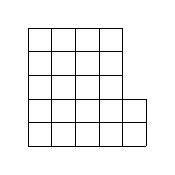
\begin{tikzpicture}[scale=0.3]
\draw (0, 0)--(0,5 );
\draw (1, 0)--(1,5 );
\draw (2, 0)--(2,5 );
\draw (3, 0)--(3,5 );
\draw (4, 0)--(4,5 );
\draw (5, 0)--(5,2 );

\draw(0,0)--(5,0);
\draw(0,1)--(5,1);
\draw(0,2)--(5,2);
\draw(0,3)--(4,3);
\draw(0,4)--(4,4);
\draw(0,5)--(4,5);
\end{tikzpicture}\]

en morceaux de forme 
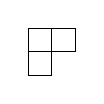
\begin{tikzpicture}[scale=0.3]
\draw(0,0)--(0,2);
\draw(1,0)--(1,2);
\draw(2,1)--(2,2);
\draw(0,0)--(1,0);
\draw(0,1)--(2,1);
\draw(0,2)--(2,2);
\end{tikzpicture}
et
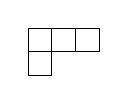
\begin{tikzpicture}[scale=0.3]
\draw(0,0)--(0,2);
\draw(1,0)--(1,2);
\draw(2,1)--(2,2);
\draw(3,1)--(3,2);
\draw(0,0)--(1,0);
\draw(0,1)--(3,1);
\draw(0,2)--(3,2);
\end{tikzpicture}.


Celle-ci est constituée de $22$ cases 
On note $x$ le nombre de morceaux de $3$ cases, et $y$ celui de ceux de $4$ cases.
On a alors $3x+4y=22$, et $x \geq 0$ et $y \geq 0$, donc $y \leq 5$.
Or $y$ est un entier, donc il n'y a que $6$ valeurs possibles de $y$:
\begin{itemize}
	\item[y=0:] Impossible car $3x=22$ avec $x$ entier
	\item[y=1:] $3x=18$ donc $x=6$
	\item[y=2:] Impossible car $3x=14$ avec $x$ entier
	\item[y=3:] Impossible car $3x=10$ avec $x$ entier
	\item[y=4:] $3x=6$ donc $x=2$
	\item[y=5:] Impossible car $3x=2$ avec $x$ entier
\end{itemize}
Ainsi les seules valeures possibles de $x$ sont $2$ et $6$.
Réciproquement, les deux figures suivantes montrent que ces $2$ valeurs conviennent effectivement.

\[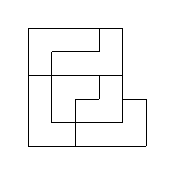
\begin{tikzpicture}[scale=0.3]
\draw (0, 0)--(0,5 );
\draw (1, 1)--(1,4 );
\draw (2, 0)--(2,2 );
\draw (3, 2)--(3,3 );
\draw (3, 4)--(3,5 );
\draw (4, 1)--(4,5 );
\draw (5, 0)--(5,2 );

\draw(0,0)--(5,0);
\draw(1,1)--(4,1);
\draw(2,2)--(3,2);
\draw(4,2)--(5,2);
\draw(0,3)--(4,3);
\draw(1,4)--(3,4);
\draw(0,5)--(4,5);
\end{tikzpicture}\]

\[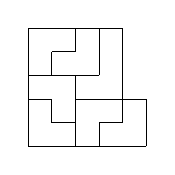
\begin{tikzpicture}[scale=0.3]
\draw (0, 0)--(0,5 );
\draw (1, 1)--(1,2 );
\draw (1, 3)--(1,4 );
\draw (2, 0)--(2,3 );
\draw (2, 4)--(2,5 );
\draw (3, 0)--(3,1 );
\draw (3, 3)--(3,5 );
\draw (4, 1)--(4,5 );
\draw (5, 0)--(5,2 );

\draw(0,0)--(5,0);
\draw(1,1)--(2,1);
\draw(3,1)--(4,1);
\draw(0,2)--(1,2);
\draw(2,2)--(5,2);
\draw(0,3)--(3,3);
\draw(1,4)--(2,4);
\draw(0,5)--(4,5);
\end{tikzpicture}\]

\end{sol}

\begin{sol}[42](Résolu par Maël Laoufi et Thibaut Desort)

Soit $x=1+\dfrac{1}{2+\dfrac{1}{2+\dfrac{1}{\cdots}}}$.

On remarque que $x=1+\dfrac{1}{1+1+\dfrac{1}{2+\dfrac{1}{\cdots}}}$, 
d'où 
\begin{eqnarray*}
x &=& 1+\frac{1}{1+x} \\
x-1 &=& \frac{1}{1+x}\\
(x+1)(x-1) &=& 1\\
x^2-1 &=& 1\\
x^2 &=& 2\\
\end{eqnarray*}

D'où $x=\sqrt{2}$ puisque $x$ est strictement positif.


\end{sol}


\begin{sol}[56](Résolu par Barthélémy Pelletier et Gaël Gallot)

Barthélémy Pelletier groupe B
Gaël Gallot groupe B

L'aire du carré est $a^2$.

L'aire du triangle est $\frac{\sqrt{3}}{4}b^2$.

On veut $a^2=\frac{\sqrt{3}}{4}b^2$, soit $a=\frac{\sqrt[4]{3}}{2}b$ car $a$ et $b$ sont strictement positifs.

Or $\frac{\sqrt[4]{3}}{2}$ est un nombre irrationnel.
Ainsi, si $b$ est rationnel, alors le produit $\frac{\sqrt[4]{3}}{2}b$ sera aussi irrationnel et $a$ sera irrationnel.

Par conséquent, $a$ et $b$ ne peuvent pas être tous les deux rationnels.

\end{sol}

\begin{sol}[22](R\'esolu par Matthias Schuller)
Le nombre $\frac{a^{2b+1}b-1}{a+1}$ doit \^etre un entier, donc $a+1$ divise $a^{2b+1}b-1$. On a donc que $a+1$ divise
\[(a^{2b+1}b-1)+(a+1)=a(a^{2b}b+1).\]
Or $a+1$ n'a aucun diviseur en commun avec $a$ car leur diff\'erence est 1, donc $a+1$ divise $a^{2b}b+1$ et donc aussi
\[(a^{2b}b+1)-(a+1)=a(a^{2b-1}b-1).\]
Par le m\^eme argument, on trouve que $a+1$ divise $a^{2b-1}b-1$. On se retrouve alors avec la formule du d\'ebut, mais avec l'exposant de $a$ diminu\'e de 2. En particulier on retrouve toujours un exposant impair. On peut alors refaire le m\^eme argument jusqu'\`a ce que l'exposant de $a$ soit \'egal \`a 1. On trouve alors que $a+1$ divise $ab-1$ et donc aussi
\[(ab-1)+(a+1)=a(b+1),\]
et donc $a+1$ doit diviser $b+1$.\\

Avec l'autre entier $\frac{b^aa+1}{b-1}$ on trouve que $b-1$ divise $b^aa+1$. On a donc que $b-1$ divise
\[(b^aa+1)+(b-1)=b(b^{a-1}a+1).\]
Toujours par le m\^eme argument, on obtient que $b-1$ divise $b^{a-1}a+1$ (noter que $b-1$ peut diviser $b$ si $b=2$, mais alors $b-1$ divise tout nombre). On se retrouve alors avec la formule du d\'ebut, mais avec l'exposant de $b$ diminu\'e de 1. Tout comme dans le cas pr\'ec\'edent, on refait l'argument jusqu'\`a ce que l'exposant de $b$ soit 0, d'o\`u on obtient finalement que $b-1$ doit diviser $a+1$.\\

On sait maintenant que $(a+1)|(b+1)$ et que $(b-1)|(a+1)$, donc $(b-1)|(b+1)$. Alors $b-1$ divise aussi
\[(b+1)-(b-1)=2,\]
ce qui nous dit que $b=2$ ou $b=3$.
\begin{itemize}
\item Si $b=2$, alors nos deux conditions d\'eviennent $(a+1)|3$ et $1|(a+1)$. Cela nous dit que $a=2$ et donc on trouve la solution $(a,b)=(2,2)$. On v\'erifie que dans ce cas on a bien des entiers :
\[\frac{2^{2\cdot 2+1}\cdot 2-1}{2+1}=21\quad\text{et}\quad\frac{2^2\cdot 2+1}{2-1}=9.\]
\item Si $b=3$, alors les deux conditions d\'eviennent $(a+1)|4$ et $2|(a+1)$. Cela nous dit que $a=1$ ou $a=3$ et donc on trouve les solutions $(a,b)=(1,3),(3,3)$. On v\'erifie aussi que dans ces cas on a bien des entiers :
\begin{align*}
\frac{1^{2\cdot 3+1}\cdot 3-1}{1+1}=1\quad&\text{et}\quad\frac{3^1\cdot 1+1}{3-1}=2.\\
\frac{3^{2\cdot 3+1}\cdot 3-1}{3+1}=1640\quad&\text{et}\quad\frac{3^3\cdot 3+1}{3-1}=41.
\end{align*}
\end{itemize}
\end{sol}

\begin{sol}[28](Résolu par Andrei Barbu)

\begin{center}
\begin{tikzpicture}[line cap=round,line join=round,>=triangle 45,scale=0.7]
\clip(-1.0,-5.0) rectangle (7.0,3.0);
\draw(3.0,-1.25) circle (3.25cm);
\draw (0.0,-0.0)-- (3.0,2.0);
\draw (3.0,2.0)-- (6.0,0.0);
\draw (0.0,-0.0)-- (6.0,0.0);
\draw (0.0,-0.0)-- (0.9942952106614191,-3.8072736064066905);
\draw (0.9942952106614191,-3.8072736064066905)-- (6.0,0.0);
\draw (3.0,2.0)-- (5.063140190852756,-0.7125633201275571);
\begin{scriptsize}
\draw (0.0,-0.0) circle (1.5pt);
\draw (-0.32,0.4000000000000011) node {$A$};
\draw (6.0,0.0) circle (1.5pt);
\draw (6.279999999999999,0.2200000000000011) node {$B$};
\draw (3.0,2.0) circle (1.5pt);
\draw (3.06,2.3600000000000008) node {$C$};
\draw (0.9942952106614191,-3.8072736064066905) circle (1.5pt);
\draw (0.8400000000000001,-4.019999999999998) node {$P$};
\draw (5.063140190852756,-0.7125633201275571) circle (1.5pt);
\draw (5.239999999999999,-0.9199999999999988) node {$D$};
\end{scriptsize}
\end{tikzpicture}
\end{center}

$ABC$ est isocèle en $C$ et $D$ est le projeté orthogonal de $C$ sur $(PB)$.
On veut montrer que $PA+PB=2\,PD$. On peut supposer que $PB > PA$ et montrer
$BD = PD - PA$. Soit $E\in (PB)$ tel que $EP = AP$. On veut montrer que
$ED=BD$, ie que $ECB$ isocèle en $C$. Or, par chasse aux angles, 
$\widehat{APC}=\widehat{ABC}=\widehat{CAB}=\widehat{CPB}$. Donc $(CP)$ est
la bissectrice issue de $P$ dans $APE$, qui est isocèle en $P$, donc c'est aussi
la médiatrice de $[AE]$. Cette médiatrice passant par $C$, $ACE$ est isocèle en $C$.
Donc $EC=AC=BC$, donc $ECB$ est bien isocèle en $C$.

\end{sol}

\begin{sol}[67](Résolu par Joris Leroy-Savin et \'Etienne Massart et d'autre part par Thomas Grenier)

Soit $E$ l'intersection de $(AQ)$ et $(PC)$. Montrons que $(DE)$ et $(PQ)$
sont perpendiculaires.

On se place dans le repère orthonormé $(D;C;A)$. Soit $0<y<1$ tel que 
$P\,(y;1)$, et donc $Q\,(1;1-y)$.
L'équation de $(AQ)$ est : $(AQ)(x)=-yx+1$, et de façon analogue : 
$(PC)(x)=-\frac{1}{1-y}x+\frac{1}{1-y}$.
On en déduit les coordonnées de $E$ : $\bigg(-\frac{y}{y-y^2-1}\,;
\frac{y^2}{y-y^2-1}+1\bigg)$, d'où $(DE)(x)=\frac{y-1}{y}x$.
On calcule aussi l'équation de $(PQ)$ : 
$(PQ)(x) = -\frac{y}{1-y}x+1-\frac{y^2}{1-y}$.
Comme le coefficient directeur de $(PQ)$ est l'opposé de l'inverse de
celui de $(DE)$, $(PQ)$ et $(DE)$ sont perpendiculaires.\\
 
\noindent{\it Autre méthode}\; En gardant la même définition du point $E$,
il s'agit de montrer que $E$ est l'orthocentre du triangle $DPQ$. Montrons
donc que $(AQ)$ est perpendiculaire à $(DP)$ et $(PC)$ à $(DQ)$. Or, comme
$AP=BQ$, $\tan(\widehat{ADP})=\tan(\widehat{BAQ})$. Ce sont des angles aigus,
donc $\widehat{ADP}=\widehat{BAQ}$. Soit $M$ le point d'intersection
de $(AP)$ et de $(BQ)$. 
On a $\widehat{AMD}=180\degres - \widehat{ADP}
 - (90\degres-\widehat{BAQ})=90\degres$. Donc $(DP)$ et $(AQ)$ sont 
 perpendiculaires, et on procède de même pour l'autre hauteur.

\end{sol}

\begin{sol}[73](R\'esolu par Guillaume Chyzak)
Consid\'erons le nombre de choix possibles pour $X$. Il y a $n\choose i$ possibilit\'es de r\'ealiser un sous-ensemble $X$ \`a $i$ \'el\'ements. Or le nombre d'\'el\'ements peut aller de 0 \`a $n$. Il y a donc $\sum_{i=0}^n {n\choose i}$ possibilit\'es.

Consid\'erons maintenant le nombre de choix possibles pour $Y$. Chacun des $i$ \'el\'ements peut \^etre pris ou non dans le sous-ensemble $Y$, ce qui donne $2^i$ possibilit\'es.

Enfin, consid\'erons le nombre de choix possibles pour $Z$. C'est un ensemble de $n-i$ \'el\'ements, donc par le m\^eme argument que pour $Y$ il y a $2^{n-i}$ possibilit\'es pour $Z$.

En mettant tout cela ensemble, on voit que le nombre de triplets $(X,Y,Z)$ est \'egal \`a
\[\sum_{i=0}^n {n\choose i} \cdot 2^i\cdot 2^{n-i}=2^n\cdot\sum_{i=0}^n {n\choose i}=2^{2n}.\]

\end{sol}

\begin{sol}[75](Résolu par Dario Shariatan)

Déterminons d'abord de combien de manières différentes il est possible de carreler un rectangle de taille $2 \times n$ avec des carreaux incolores. Notons $F(n)$ ce nombre.

Pour les rectangles de taille $2 \times 1$ ou $2 \times 2$ on voit aisément que :
\begin{itemize}
\item Il n'y a qu'une seule façon de carreler le rectangle $2\times 1$
\item Il y a deux façons de carreler le rectangle $2 \times 2$ (carreaux horizontaux ou verticaux)
\end{itemize}

Pour carreler un carreau de taille $2 \times (n+1)$ il n'y a qu'une seule manière de s'y prendre :
\begin{itemize}
\item Soit on commence par un carreau $2 \times 1$ au début du rectangle et on carrele le rectangle de taille $2 \times (n-1)$ restant, il y a $F(n-1)$ possibilités
\item Soit on commence par deux carreaux $1 \times 2$ et on a $F(n-2)$ possibilités pour compléter le rectangle.
\end{itemize}

On a donc la relation de récurrence $F(n) = F(n-1) + F(n-2)$.

Étudions maintenant l'influence des couleurs. Pour carreler un rectangle, on utilise $n$ carreaux, qui peuvent chacun être colorés de deux manières différentes. Considérons un carrelage incolore donné, comme la position des carreaux est importante, il y a $2^n$ manières de colorier cette disposition. 

Ainsi, le nombre de manières de carreler un rectangle $2 \times n$ est $2^n \times F(n)$ où $F(n)$ est le $(n+1)$-ième terme de la suite de Fibonacci.

\end{sol}

\begin{sol}[79](Résolu par Timothée Roquet et Théodore Fougereux)
 
Si $p = 2$, l'équation devient $3=q(2+q^2)$, donc $q$ divise $3$ et, comme $q$ est premier $q = 3$, ce qui est absurde.
De même, si $q = 2$, l'équation devient $p(p-2) = 9$, donc $p$ divise $9$, puis $p = 3$, ce qui est aussi absurde.
On sait donc que $p$ et $q$ sont des nombres premiers impairs.
 
On réécrit alors l'équation $p^2-pq-q^3=1$ sous la forme
$(p-1)(p+1) = q(p+q^2)$, ou encore sous la forme $p(p-q) = (q+1)(q^2-q+1)$.
Puisque $q \mid p-1$ ou $q \mid p+1$, on sait que $q \leq \frac{p+1}{2}$.
Par conséquent, si $p \mid q+1$, on a $p \leq \frac{q+1}{2} \leq \frac{p+3}{4}$, c'est-à-dire $p \leq 1$, ce qui est absurde.
On sait donc que $p \mid q^2-q+1$.

Si $q \mid p+1$, soit $n$ l'entier tel que $p+1 = nq$. Puisque $p$ et $q$ sont impairs, $n$ est pair, donc $n \geq 2$.
Alors $nq-1 = p \leq q^2-q+1$, donc $n \leq q-1 + \frac{2}{q} < q$,
et $n \leq q-1$. Puis $0 \equiv q^2-q+1 \equiv q^2-q+1+(nq-1) \equiv q(q+n-1) \pmod{nq-1}$.
Puisque $q$ est premier avec $q < 2q-1 \leq nq-1$, les entiers $q$ et $nq-1$ sont premiers entre eux, donc $nq-1 \mid q+n-1$.
Or, on a $nq - n - q + 1 = (q-1)(n-1) \geq 2$, donc
$0 < q+n-1 < nq-1$, et $nq-1$ ne peut pas diviser $q+n-1$.

Il faut donc que $q \mid p-1$. Soit $n$ l'entier tel que $p-1 = nq$. Comme précédemment, $nq+1 = p \leq q^2-q+1$, donc $n \leq q-1$.
Puis $0 \equiv q^2-q+1 \equiv q^2-q+1-(nq+1) \equiv q(q-1-n) \pmod{nq+1}$. Comme $q$ est premier avec $q < nq+1$,
les entiers $q$ et $nq+1$ sont premiers entre eux, donc $nq+1 \mid q-1-n$. Puisque $0 \leq q-1-n < nq+1$, il
faut nécessairement avoir $q-1-n = 0$, c'est-à-dire $n = q-1$ et $p = q^2-q+1$.

L'équation de départ, qui est $p(p-q) = (q+1)(q^2-q+1)$, est donc équivalente à $p-q = q+1$, ou encore à $q(q-1)+1 = q^2-q+1 = p = 2q+1$.
Il faut donc nécessairement avoir $q = 3$, puis $p = 7$, et alors on a bien $p^2-pq-q^3 = 49 - 21 - 27 = 1$.
L'unique solution du problème est donc obtenue pour $p = 7$ et $q = 3$.
\end{sol}

\begin{sol}[82](R\'esolu par Thimot\'ee Roquet et Th\'eodore Fougereux)
Pour $n\in\N$, notons $S_n=\sum_{i=0}^n x_i$. On d\'emontre par r\'ecurrence l'affirmation
\begin{center}
$P_n:$ {\it il existe un entier $m$ tel que $S_n=\frac{m(m+1)}{2}$.}
\end{center} 

\paragraph*{Initialisation} Pour $n=0$, on a par hypoth\`ese $x_0^2=x_0^3$, ce qui est \'equivalent \`a $x_0^2(x_0-1)=0$, donc $x_0=0$ ou $x_0=1$. Dans les deux cas, on voit qu'en posant $m=x_0$ on a $S_0=x_0=\frac{m(m+1)}{2}$, ce qui conclut dans ce cas.

\paragraph*{H\'er\'edit\'e} On suppose que l'on a la propri\'et\'e $P_n$, donc $S_n=\frac{m(m+1)}{2}$ pour un certain entier $m$. On doit trouver un entier $m'$ tel que $S_{n+1}=\frac{m'(m'+1)}{2}$. Par hypoth\`ese, on sait que
\[x_1^3+\cdots+x_n^3=S_n^2\quad\text{et}\quad x_1^3+\cdots+x_{n+1}^3=S_{n+1}^2.\]
De cela on d\'eduit
\[x_1^3+\cdots+x_{n+1}^3-(x_1^3+\cdots+x_{n}^3)=S_{n+1}^2-S_n^2=(S_n+x_{n+1})^2-S_n^2,\]
et donc finalement,
\[x_{n+1}^3=x_{n+1}(2S_n+x_{n+1}).\]

Supposons d'abord que $x_{n+1}=0$. Alors dans ce cas on a $S_{n+1}=S_n=\frac{m(m+1)}{2}$ d'apr\`es $P_n$ et alors $P_{n+1}$ est v\'erifi\'ee pour l'entier $m'=m$. Sinon, on peut diviser la derni\`ere \'equation par $x_{n+1}$ pour trouver $x_{n+1}^2=2S_n+x_{n+1}$, ou encore $S_n=\frac{x_{n+1}(x_{n+1}-1)}{2}$.

Posons $X=x_{n+1}-1$. Alors $S_n=\frac{X(X+1)}{2}$, mais aussi $S_n=\frac{m(m+1)}{2}$ d'apr\`es  $P_n$, donc \[X^2+X=m^2+m,\]
et alors
\[0=X^2+X -m^2+m=\left(X^2+X+\frac14\right) -\left(m^2+m+\frac14\right)=\left(X+\frac12\right)^2-\left(m+\frac12\right)^2,\]
et finalement
\[(X+m+1)(X-m)=0,\]
ce qui nous dit que $X=m$ ou $X=-m-1$. Et en rappelant que $X=x_{n+1}-1$, on trouve que $x_{n+1}=m+1$ ou $x_{n+1}=-m$.

Si $x_{n+1}=m+1$, alors $S_{n+1}=S_n+x_{n+1}=\frac{m(m+1)}{2}+m+1=\frac{(m+1)(m+2)}{2}$, donc $P_{n+1}$ est v\'erifi\'ee pour l'entier $m'=m+1$.

Si $x_{n+1}=-m$, alors $S_{n+1}=S_n+x_{n+1}=\frac{m(m+1)}{2}-m=\frac{(m-1)m}{2}$, donc $P_{n+1}$ est v\'erifi\'ee pour l'entier $m'=m-1$.

\end{sol}

\begin{sol}[83](R\'esolu par Timoth\'ee Roquet et Th\'eodore Fougereux)
On a
\[\frac{x}{x+2y+3z}+\frac{y}{y+2z+3x}+\frac{z}{z+2x+3y}=\frac{x^2}{x^2+2xy+3xz}+\frac{y^2}{y^2+2yz+3xy}+\frac{z^2}{z^2+2xz+3yz},\]
et en appliquant l'in\'egalit\'e des mauvais \'el\`eves au terme de droite on trouve
\[\frac{x}{x+2y+3z}+\frac{y}{y+2z+3x}+\frac{z}{z+2x+3y}\geq \frac{(x+y+z)^2}{x^2+y^2+z^2+5(xy+xz+yz)}.\]
Il suffit alors de montrer
\[\frac{(x+y+z)^2}{x^2+y^2+z^2+5(xy+xz+yz)}\geq \frac12,\]
ce qui est \'equivalent \`a
\begin{align*}
2(x+y+z)^2 &\geq x^2+y^2+z^2+5(xy+xz+yz)\\
2x^2+2y^2+2z^2+4xy+4xz+4yz &\geq x^2+y^2+z^2+5(xy+xz+yz)\\
x^2+y^2+z^2 &\geq xy+xz+yz.
\end{align*}
Sans perte de g\'en\'eralit\'e, on peut supposer que $x\geq y\geq z$. La derni\`ere in\'egalit\'e correspond alors \`a l'in\'egalit\'e de r\'eordonnement, ce qui conclut.

\end{sol}

\begin{sol}[97](Résolu par Baptiste Serraille)

On veut montrer que cinq droites rouges sont concourantes. Comme le problème est d\'efini de manière cyclique, il nous suffira de montrer que trois droites cons\'ecutives le sont. 

On va montrer ceci par la m\'ethode dynamique de g\'eom\'etrie projective suivante : 
on d\'efinit une transformation projective d'un espace unidimensionnel projectif sur lui-même (comme compos\'ee de transformations projectives \'el\'ementaires). Si l'\'enonc\'e final est vrai, cette transformation devrait être l'identit\'e (elle est construite dans cette optique). Or, \'etant une transformation projective, il suffira de montrer qu'elle est bien l'identit\'e pour trois points distincts de l'espace de d\'efinition pour montrer qu'elle est bien l'identit\'e sur tout l'espace. 

En pratique, on fixe les points B, F, I, Y, H, J, E et donc les cercles circonscrits à IYFB, IYHJ et les droites (IY), (IHE), (JHFB), (BCE) et (IFC). On fait varier un point $P_1$ sur la droite (IY). Les projections suivantes sont des transformations projectives : $P_1$ est envoy\'e sur X, X est envoy\'e sur A, A est envoy\'e sur G, G est envoy\'e sur Z et Z est envoy\'e sur $P_2$ (point d'intersection de (JZ) et (IY)). 

Il suffit maintenant de montrer que $P_1=P_2$ pour $3$ positions distinctes de $P_1$. Or $P_1=I$ et $P_1=(BFHJ)\cap (IY)$ sont des cas faciles. La troisième position qui correspond à $A = \infty$ (de la droite (IFC)) se montre en r\'eit\'erant la même m\'ethode projective que pr\'ec\'edemment. 
	
\end{sol}

\begin{sol}[100](Résolu par Pierre-Alexandre Bazin)
 
Pour tout $k \geq 0$, on note $(a_{k,1},\ldots,a_{k,n})$ les coefficients du $n$-uplets $T^k(a_1,\ldots,a_n)$.
Soit $M_k$ le maximum des réels $a_{k,1},\ldots,a_{k,n}$, $A_k$ le nombre d'indices $i$ tels que $a_{k,i} = M_k$,
et $X_k$ la moyennne des réels $a_{k,1},\ldots,a_{k,n}$.
Il est clair que $X_k = X_{k+1}$ pour tout $k \geq 0$.
On suppose maintenant que, pour tout entier $k \geq 0$, les entiers $a_{k,1},\ldots,a_{k,n}$ ne sont pas tous égaux et sont tous entiers.
D'autre part, on considèrera les indices $i$ modulo $n$ (on pourra donc noter $n+1$ pour l'indice $1$, etc).

Montrons que, pour tout $k \geq 0$, on a soit $M_{k+1} < M_k$, soit $M_{k+1} = M_k$ et $A_{k+1} < A_k$.
En effet, on a $2 a_{k+1,i} = a_{k,i} + a_{k,i+1} \leq 2 M_k$ pour tout $i$, donc $M_{k+1} \leq M_k$.
Puis, si $M_{k+1} = M_k$, alors on doit avoir $a_{k,i} = a_{k,i+1} = M_k$ pour tout $i$ tel que $a_{k+1,i} = M_k$.
Par conséquent, si les $a_{k,i}$ ne sont pas tous égaux, il existe un entier $i$ tel que
$a_{k,i} = M_k > a_{k,i+1}$, donc $a_{k+1,i} < M_k$.
Il s'ensuit que $A_{k+1} < A_k$.

La suite $(M_k)_{k \geq 0}$ est décroissante, à valeurs entières, et minorée par $X_0$, donc elle converge en une valeur $M_\kappa$.
Puis la suite $(A_k)_{k \geq \kappa}$ est strictement décroissante, et à valeurs entières positives, ce qui est impossible.
Sous réserve que les $a_{k,i}$ soient tous entiers quels que soient $k$ et $i$, il existe donc un entier $\kappa$ tel que
$a_{\kappa,1} = \ldots = a_{\kappa,n} = M_\kappa$.
Sans perte de généralité, quitte à soustraire $M_\kappa$ à tous les entiers $a_i$, on suppose que $M_\kappa = 0$.

Maintenant, intéressons-nous aux $n$-uplets $(x_1,\ldots,x_n)$ tels que $T(x_1,\ldots,x_n) = (0,\ldots,0)$.
On a toujours $x_i + x_{i+1} = 0 = x_{i+1} + x_{i+2}$.
Par conséquent, si $n$ est impair, on a $x_1 = x_3 = \ldots = x_n = x_2 = x_4 = \ldots = x_{n-1} = 0$.
Le $n$-uplet $(0,\ldots,0)$ n'a donc d'autre antécédent par $T$ que lui-même, et puisque
les entiers $a_1,\ldots,a_n$ sont deux à deux distincts, il est impossible d'avoir $T^k(a_1,\ldots,a_n) = (0,\ldots,0)$,
quel que soit l'entier $k$ considéré.

Si $n$ est pair, en revanche, tout antécédent de $(0,\ldots,0)$ est de la forme $(x,-x,x,-x,\ldots,x,-x)$, où $x$ est un réel.
Puis tout antécédent de $(x,-x,x,-x,\ldots,x,-x)$ est nécessairement de la forme
$(y,2x-y,y-4x,6x-y,y-8x,\ldots,nx-y)$, où $y$ est un réel tel que $2nx = 2x$. Puisque $n > 2$, un tel antécédent n'existe que si $x = 0$,
mais lui-même est de la forme $(y,-y,y,-y,\ldots,y,-y)$.
Par conséquent, là aussi, puisque les entiers $a_1,\ldots,a_n$ sont deux à deux distincts, il est impossible d'avoir $T^k(a_1,\ldots,a_n) = (0,\ldots,0)$,
quel que soit l'entier $k$ considéré.

Notre supposition selon laquelle les $a_{k,i}$ soient tous entiers quels que soient $k$ et $i$ était donc fausse, ce qui conclut l'exercice.
\end{sol}

\begin{sol}[102](Résolu par Olivier Garçonnet)
On va montrer que $n = 7$.
On montre d'abord, par récurrence sur le nombre $k$ de députés,
que séparer les députés en $7$ groupes (éventuellement vides) est toujours faisable.
Si $k \geq 7$, c'est évident. Ensuite, si $k \geq 8$, un député étant détesté
par $3$ collègues en moyenne, il existe nécessairement un député détesté par au plus $3$ collègues.
Appelons-le X, et excluons-le temporairement.

Par hypothèse de récurrence, on peut répartir les $k-1$ députés restants en $7$ groupes.
Au plus $6$ de ces groupes contiennent un député qui déteste ou est détesté par X.
On peut donc mettre X dans le groupe restant (ou un des groupes restants),
ce qui montre bien que l'on peut en fait répartir convenablement n'importe quelle famille de $k$ députés.
Cela conclut la récurrence, montrant que $n \geq 7$.

D'autre part, considérons six députés $X_0,\ldots,X_6$.
Supposons que chaque député $X_i$ déteste les députés $X_j$ avec $j-i \in \{1,2,3\} \pmod{6}$.
Alors on ne peut jamais mettre deux députés dans un même groupe, donc il nous faut au moins $7$ groupes.
Cela montre que $n \geq 7$, donc que $n = 7$.
\end{sol}

\begin{sol}[105](Résolu par Yakob Kahane)

On va montrer que Alice gagne dans le deuxième cas, et donc dans le premier.
Pour ce faire, elle va peindre en rouge des motifs particuliers sur les deux diagonales $\{(n,n) \mid n \in \Z\}$ et $\{(n,1-n) \mid n \in \Z\}$.

Soit $k \geq 1$ un entier. Supposons qu'il existe deux abscisses $x$ et $x+k$ telles qu'Alice ait colorié en rouge les quatre cases
$(x,x)$, $(x+k,x+k)$, $(x,1-x)$ et $(x+k,1-x-k)$ : on dit que la paire $(x,x+k)$ est une $k$-abscisse.
De même, s'il existe deux ordonées $y$ et $y+k$ telles que les quatre cases $(y,y)$, $(y+k,y+k)$, $(1-y,y)$ et $(1-y-k,y+k)$
soient rouges, on dit que la paire $(y,y+k)$ est une $k$-ordonnée.

Supposons maintenant que $(x,x+k)$ est une $k$-paire et que $(y,y+k)$ est une $k$-ordonnée, avec $x \geq k+2$, $y \geq k+2$ et $|x - y| \geq k+2$.
Alors les entiers $x$, $1-x$, $x+k$, $1-x-k$, $y$, $1-y$, $y+k$ et $1-y-k$ sont distincts deux à deux.
On note alors $\mathcal{D}^k_{x,y}$ et $\mathcal{E}^k_{x,y}$ les ensembles de cases définis comme suit :
\[\mathcal{D}^k_{x,y} = \{(x,y),(y,x),(1-y,1-x)\} \text{ et } \mathcal{E}^k_{x,y} = \mathcal{D}^k_{x,y} \cup \mathcal{D}^k_{x+k,y} \cup \mathcal{D}^k_{x,y+k} \cup \{(x+k,y+k)\}.\]

Si Bob n'a colorié en vert aucune case de $\mathcal{D}^k_{x,y}$, alors Alice colorie en rouge la case $(x,y)$.
Bob doit empêcher les deux carrés $(x,y)$, $(x,x)$, $(y,y)$, $(y,x)$ et
$(x,y)$, $(x,1-x)$, $(1-y,y)$, $(1-y,1-x)$ de devenir entièrement rouges : il doit donc jouer tout de suite en $(y,x)$ et en $(1-y,1-x)$.
Alors Alice joue en $(x+k,y)$ : Bob répond alors en $(y,x+k)$ et en $(1-y,1-x-k)$. Puis elle joue en $(y+k,x)$ : Bob répond en
$(y+k,x)$, $(1-y-k,1-x)$. Enfin, Alice joue en $(x+k,y+k)$ pour obtenir un carré rouge et ainsi gagner.
Bob doit donc nécessairement avoir déjà colorié une case en bleu de l'ensemble $\mathcal{D}^k_{x,y}$, sous peine de perdre.

\begin{center}
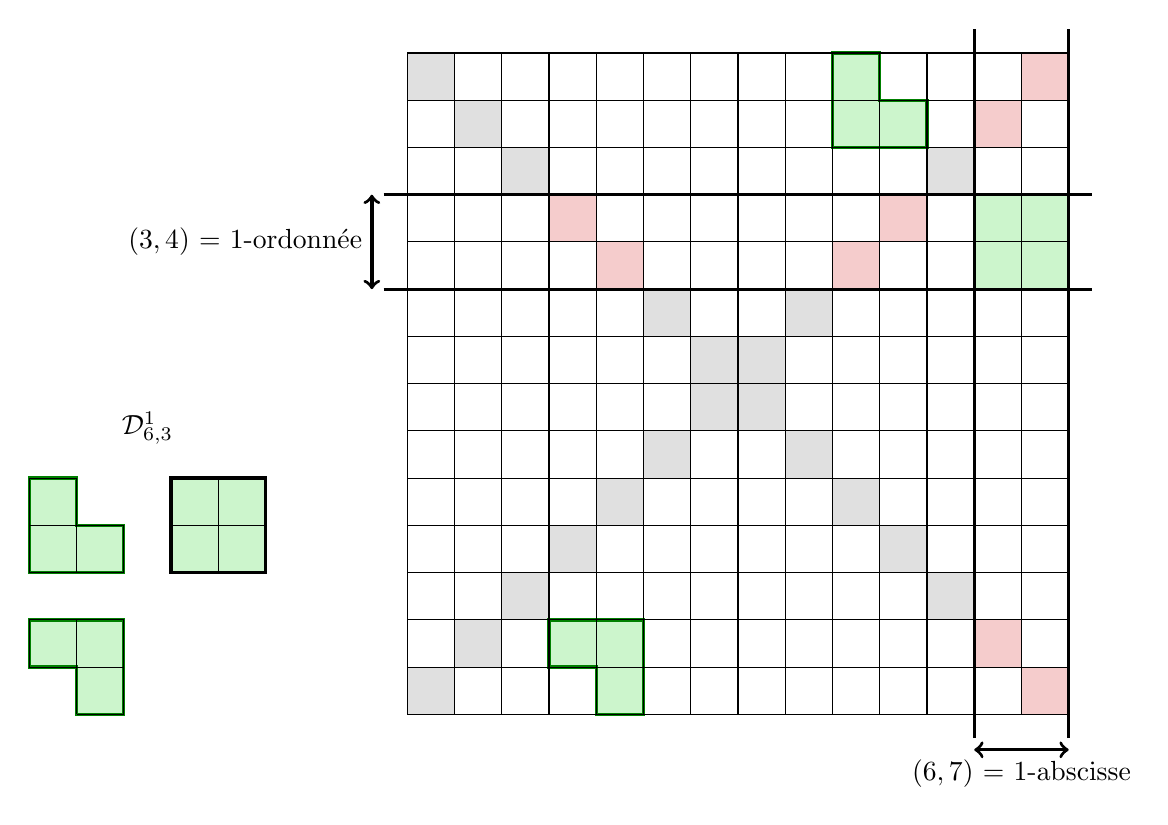
\begin{tikzpicture}[scale=0.6]
\newcommand{\fillcase}[3]{\draw[fill=black!20!#1!20] (#2,#3) -- (#2,#3-1) -- (#2-1,#3-1) -- (#2-1,#3) -- cycle;}

\fillcase{red}{7}{7}
\fillcase{red}{6}{6}
\fillcase{gray}{5}{5}
\fillcase{red}{4}{4}
\fillcase{red}{3}{3}
\fillcase{gray}{2}{2}
\fillcase{gray}{1}{1}
\fillcase{gray}{0}{0}
\fillcase{gray}{-1}{-1}
\fillcase{gray}{-2}{-2}
\fillcase{gray}{-3}{-3}
\fillcase{gray}{-4}{-4}
\fillcase{gray}{-5}{-5}
\fillcase{gray}{-6}{-6}

\fillcase{red}{7}{-6}
\fillcase{red}{6}{-5}
\fillcase{gray}{5}{-4}
\fillcase{gray}{4}{-3}
\fillcase{gray}{3}{-2}
\fillcase{gray}{2}{-1}
\fillcase{gray}{1}{0}
\fillcase{gray}{0}{1}
\fillcase{gray}{-1}{2}
\fillcase{red}{-2}{3}
\fillcase{red}{-3}{4}
\fillcase{gray}{-4}{5}
\fillcase{gray}{-5}{6}
\fillcase{gray}{-6}{7}

\fillcase{green}{6}{3}
\fillcase{green}{3}{6}
\fillcase{green}{-2}{-5}
\fillcase{green}{7}{3}
\fillcase{green}{3}{7}
\fillcase{green}{-2}{-6}
\fillcase{green}{6}{4}
\fillcase{green}{4}{6}
\fillcase{green}{-3}{-5}
\fillcase{green}{7}{4}

\draw[very thick,draw=black!50!green] (3,7) -- (2,7) -- (2,5) -- (4,5) -- (4,6) -- (3,6) -- cycle;
\draw[very thick,draw=black!50!green] (-2,-7) -- (-2,-5) -- (-4,-5) -- (-4,-6) -- (-3,-6) -- (-3,-7) -- cycle;

\draw (-7,-7) -- (7,-7);
\draw (-7,-6) -- (7,-6);
\draw (-7,-5) -- (7,-5);
\draw (-7,-4) -- (7,-4);
\draw (-7,-3) -- (7,-3);
\draw (-7,-2) -- (7,-2);
\draw (-7,-1) -- (7,-1);
\draw (-7,0) -- (7,0);
\draw (-7,1) -- (7,1);
\draw[very thick] (-7.5,2) -- (7.5,2);
\draw (-7,3) -- (7,3);
\draw[very thick] (-7.5,4) -- (7.5,4);
\draw (-7,5) -- (7,5);
\draw (-7,6) -- (7,6);
\draw (-7,7) -- (7,7);

\draw (-7,-7) -- (-7,7);
\draw (-6,-7) -- (-6,7);
\draw (-5,-7) -- (-5,7);
\draw (-4,-7) -- (-4,7);
\draw (-3,-7) -- (-3,7);
\draw (-2,-7) -- (-2,7);
\draw (-1,-7) -- (-1,7);
\draw (0,-7) -- (0,7);
\draw (1,-7) -- (1,7);
\draw (2,-7) -- (2,7);
\draw (3,-7) -- (3,7);
\draw (4,-7) -- (4,7);
\draw[very thick] (5,-7.5) -- (5,7.5);
\draw (6,-7) -- (6,7);
\draw[very thick] (7,-7.5) -- (7,7.5);

\draw[very thick,<->] (-7.75,2) -- (-7.75,4);
\node[anchor=east] at (-7.75,3) {$(3,4)$ = $1$-ordonnée};
\draw[very thick,<->] (5,-7.75) -- (7,-7.75);
\node[anchor=north] at (6,-7.75) {$(6,7)$ = $1$-abscisse};

\draw[very thick,draw=black!50!green,fill=black!20!green!20!white] (-13,-7) -- (-13,-5) -- (-15,-5) -- (-15,-6) -- (-14,-6) -- (-14,-7) -- cycle;
\draw[very thick,draw=black!50!green,fill=black!20!green!20!white] (-14,-2) -- (-15,-2) -- (-15,-4) -- (-13,-4) -- (-13,-3) -- (-14,-3) -- cycle;
\draw[very thick,fill=black!20!green!20!white] (-10,-2) -- (-12,-2) -- (-12,-4) -- (-10,-4) -- cycle;
\draw (-10,-2) -- (-10,-4);
\draw (-11,-2) -- (-11,-4);
\draw (-12,-2) -- (-12,-4);

\draw (-13,-3) -- (-13,-4);
\draw (-14,-2) -- (-14,-4);
\draw (-15,-2) -- (-15,-4);
\draw (-13,-5) -- (-13,-7);
\draw (-14,-5) -- (-14,-7);
\draw (-15,-5) -- (-15,-6);

\draw (-10,-2) -- (-12,-2);
\draw (-10,-3) -- (-12,-3);
\draw (-10,-4) -- (-12,-4);

\draw (-14,-2) -- (-15,-2);
\draw (-13,-3) -- (-15,-3);
\draw (-13,-4) -- (-15,-4);
\draw (-13,-5) -- (-15,-5);
\draw (-13,-6) -- (-15,-6);
\draw (-13,-7) -- (-14,-7);

\node[anchor=south] at (-12.5,-1.5) {$\mathcal{D}^1_{6,3}$};
\end{tikzpicture}
\end{center}

L'idée de la stratégie d'Alice est la suivante : si elle réussit, pour deux entiers $k$ donnés et $K$ donnés, mais pour un entier $n$ arbitrairement grand, à créer
en $K n$ coups $n$ paires $(x,x+k)$ qui soient des $k$-abscisses et $n$ paires $(y,y+k)$ qui soient des $k$-ordonnées,
alors Bob aura dû colorier, durant ces $K n$ coups que joue Alice (donc $2 K n$ coups que joue Bob),
des cases parmi $n^2$ ensembles $\mathcal{D}_{x,y}^k$ deux à deux disjoints. Pour $n$ suffisamment grand, à $K$ fixé, Alice pourra donc gagner.

\medskip

Soit donc $n$ un entier naturel non nuls, arbitrairement grand. On pose
$R = 306 (n+1)$, $Q = 12 R+1$ et $P = \binom{15}{5} Q$.

Tout d'abord, Alice procède en $P$ étapes. Lors de chaque étape, elle joue $6$ coups, comme suit.
Alice choisit un entier positif $a \geq 1$ tel que nulle case de l'ensemble $\mathcal{F}_a = \{(x,x) \mid 16 a \leq x \leq 16 a + 15\}$ ne soit encore coloriée.
Puis, lors des $6$ prochains coups, elle colorie une des $16$ cases de cette ensemble, en commençant par la case $(16 a,16 a)$.
Au moment de jouer le dernier coup, au plus $15$ cases
de l'ensemble auront été coloriées en rouge ou en bleu, donc Alice peut bien se débrouiller pour colorier $6$ cases parmi celles de $\mathcal{F}_a$.

D'après le principe des tiroirs,
après avoir effectué ces $P$ étapes, il existera nécessairement un ensemble
$\mathcal{S} \subseteq \{0,1,\ldots,16\}$ de cardinal $6$
tel que $0 \in \mathcal{S}$ et tel que, pour (au moins) $Q$ valeurs de $a$, Alice a colorié les cases
$\{(x,x) \mid x - 16 a \in \mathcal{S}\}$. On note $\mathcal{A}$ l'ensemble de ces $Q$ valeurs de $a$.

Puis, quitte à translater le repère (et donc l'ensemble $\mathcal{A}$), on suppose que nulle case
de la seconde diagonale $\{(x,1-x) \mid x \in \Z\}$ n'a encore été coloriée, et que $\mathcal{A} \subseteq \N^\ast$.
On appelle cet instant \og{}instant critique\fg{} de la stratégie d'Alice.
Alice procède ensuite en $R$ étapes.
Pour chaque valeur non nulle $s \in \mathcal{S}$, elle initialise un compteur $\mathbf{C}(s)$ à la valeur $0$.

Lors de chaque étape, Alice joue $2$ coups, comme suit.
Elle choisit un entier $a \in \mathcal{A}$ tel que nulle case de l'ensemble $\{(x,1-x) \mid x - 16 a \in \mathcal{S}\}$ ne soit encore coloriée.
Au plus $6 R$ cases ont été coloriées depuis l'instant critique, et puisque $6 R < Q$, il existe bien un tel entier $a$.
Alors Alice colorie en rouge la case $(16a,1-16a)$, puis Bob colorie en bleu $2$ cases, et alors il reste au moins $3$ entiers $s \in \mathcal{S}$
tels que la case $(16a+s,1-16a-s)$ ne soit pas coloriée. Parmi ces entiers, Alice en choisit un tel que le compteur $\mathbf{C}(s)$ soit minimal,
elle colorie en rouge la case $(16a+s,1-16a-s)$, et elle incrémente la valeur de $\mathcal{C}(s)$.

Par conséquent, après $R$ étapes, nul compteur $\mathbf{C}(s)$ ne peut dépasser la valeur $\frac{R}{3}$,
et il y a donc au moins $3$ valeurs non nulles de $s \in \mathcal{S}$ telles que $\mathbf{C}(s) \geq \frac{R}{9} = 34 (n+1)$.
En particulier, pour chacune de ces $3$ valeurs de $s$ (disons $s_1$, $s_2$ et $s_3$),
Alice vient de créer au moins $34 (n+1)$ paires $(16a,16a+s)$ qui sont des $s$-abscisses.

Alice procède une dernière fois en $R$ nouvelles étapes, de manière analogue,
mais en se concentrant sur les ensembles $\{(1-x,x) \mid x - 16 a \in \mathcal{S}\}$.
Là encore, au plus $12 R$ cases ont été coloriées depuis l'instant critique, et puisque $12 R < Q$, des entiers $a$ convenables existent bien.
À la fin de ces $R$ nouvelles étapes, il existe au moins $3$ valeurs de $s$ (disons $s_4$, $s_5$ et $s_6$) telles qu'Alice
a créé au moins $34 (n+1)$ paires $(16a,16a+s)$ qui sont des $s$-ordonnées.
On atteint alors l'instant \og{}final\fg{} de la stratégie d'Alice.

Les deux ensembles $\{s_1,s_2,s_3\}$ et $\{s_4,s_5,s_6\}$ sont inclus dans $\mathcal{S} \setminus \{0\}$, donc s'intersectent.
Il existe donc une valeur non nulle $s \in \mathcal{S}$ telle qu'au moins $34 (n+1)$ de nos $s$-abscisses et $34 (n+1)$ de nos $s$-ordonnées ont été créées.
Puisque l'on sait que $s+2 \leq 17$, on peut sélectionner $n$ de nos $s$-abscisses, par exemple $(x_1,x_1+s),\ldots,(x_n,x_n+s)$, et
$n$ de nos $s$-abscisses, par exemple $(y_1,y_1+s),\ldots,(y_n,y_n+s)$, telles que l'on ait $x_i \geq s+2$, $y_i \geq s+2$ et $|x_i-y_j| \geq s+2$ pour tous $i, j$.

Mais alors chaque choix des paires $(x_i,x_i+s)$ et $(y_j,y_j+s)$ satisfait les conditions mentionnées en début de solution,
et les ensembles $\mathcal{D}^s_{x_i,y_j}$ sont deux à deux disjoints.
Or, cet instant final a été atteint après qu'Alice a joué $6P + 4R = 6 \binom{15}{5} (76 \cdot 306 n + 312)$ coups,
et pour éviter une défaite assurée il faut que Bob ait colorié des cases dans chacun des $n^2$ ensembles $\mathcal{D}^s_{x_i,y_j}$.
Il n'a eu le temps de colorier qu'un total de $12 \binom{15}{5} (76 \cdot 306 n + 312)$ cases, ce qui est strictement plus petit que $n^2$ quand $n$ est
suffisamment grand.

Il s'ensuit qu'Alice dispose bien d'une stratégie gagnante, même si Bob s'autorise à jouer $2$ coups après chacun des coups d'Alice.

\begin{sol}[116](R\'esolu par Martin Rakovsky et Savinien Kreczman)
Si $x\leq-5$, on a
\[y^2=x^3+(x+4)^2<x^3+x^2=x^2(x+1)<0,\]
ce qui est absurde. Par un calcul direct, on trouve aussi $y^2<0$ pour $x=-4,-3,-2$. Enfin, pour $x=-1$, on trouve $y^2=8$, ce qui est aussi absurde.

Pour $x=0$, on trouve $y^2=16$, ce qui donne les premiers couples de solutions $(0,4)$ et $(0,-4)$. On peut alors supposer d\'esormais que $x\geq 1$.\\

En regardant l'\'equation modulo 2, on d\'ecouvre que $y$ doit \^etre pair. En passant le $(x+4)^2$ de l'autre c\^ot\'e et en factorisant, on trouve
\begin{equation*}\label{eq1}
x^3=(y-x-4)(y+x+4).\tag{1}
\end{equation*}
Si $x$ est une puissance de 2, alors $y-x-4$ et $y+x+4$ sont aussi des puissances de 2. Il existe alors $a,b\in\N$ tels que
\[x=2^{\frac{a+b}{3}},\qquad y+x+4=2^a,\qquad y-x-4=2^b.\]
Alors,
\begin{align*}
(y+x+4)-(y-x-4) &=2x+8,\\
2^a-2^b&=2\cdot 2^{\frac{a+b}{3}}+8,\\
2^a&=2^{\frac{a+b}{3}+1}+2^b+8.
\end{align*}
Si $b\geq 6$, on a
\[2^a=2^{\frac{a+b}{3}+1}+2^b+8\geq 2^{\frac{a}{3}+3}+2^6+8,\]
qui est un multiple de 8. Donc
\[2^a=2^3(2^{\frac{a+b}{3}-3}+2^{b-3}+1).\]
Or, $2^{\frac{a+b}{3}-3}+2^{b-3}+1$ est impair, sauf si $a=3$ et $b=6$, mais l\`a on obtient $8=80$, ce qui est absurde. On obtient alors une contradiction pour $b\geq 6$. Et par des calculs directs, on v\'erifie que pour $1\leq b\leq 5$ on n'obtient pas des solutions non plus.\\

On peut alors supposer que $x$ admet un diviseur impair. Soit $p$ un nombre premier impair divisant $x$. Alors $p|x^3$ et donc $p|(y-x-4)$ ou bien $p|(y+x+4)$. Mais si $p$ divise les deux nombres en m\^eme temps on trouve que $p$ divise leur somme qui est \'egale \`a $2x+8$, donc $p$ divise $8$ et $p=2$, ce qui est absurde. Donc tout diviseur premier $q$ de $x$ divise soit $y-x-4$ ou $y+x+4$ mais pas les deux. D'apr\`es l'\'equation \eqref{eq1}, il existe alors $a,b,c,d\in\N$, avec $c$ et $d$ impairs et premiers entre eux, tels que
\[x=2^{\frac{a+b}{3}}cd,\qquad y+x+4=2^ac^3,\qquad y-x-4=2^bd^3.\]
Alors,
\begin{align*}
(y+x+4)-(y-x-4) &=2x+8,\\
2^ac^3-2^bd^3&=2^{\frac{a+b}{3}+1}cd+8.\tag{2}\label{eq2}
\end{align*}
On va montrer maintenant que $2^ac^3$ et $2^bd^3$ sont tous les deux des cubes. Autrement dit, on va montrer que $3|a$ et $3|b$. Or, on a \'evidemment que $3|(a+b)$ car sinon $x$ n'est pas un entier. On regarde alors diff\'erents cas :
\begin{itemize}
\item Si $a+b=0$, alors $a=b=0$ et on a conclu.
\item Si $a+b=3$, alors le c\^ot\'e droit de \eqref{eq2} est un multiple de 4, mais pour les 4 diff\'erents choix de $a$ et $b$ on voit que le c\^ot\'e gauche ne l'est pas, ce qui est absurde.
\item Si $a+b=6$, alors le c\^ot\'e droit de \eqref{eq2} est un multiple de 8. Pour que le c\^ot\'e gauche le soit aussi il faut alors $a=b=3$, ce qui conclut dans ce cas.
\item Si $a+b\geq 9$, alors le c\^ot\'e droit de \eqref{eq2} est congru \`a $8\mod 16$. De plus, on a que l'un des nombres $a$ et $b$ est $\geq 5$. Pour avoir un c\^ot\'e gauche congru \`a $8\mod 16$ il faut alors que l'autre nombre soit \'egal \`a $3$. On retrouve alors que tous les deux sont des multiples de 3, ce qui conclut dans ce dernier cas.\\
\end{itemize}

D'apr\`es ce qui pr\'ec\`ede, il existe $m,n\in\N$ tels que $m^3=2^ac^3$ et $n^3=2^bd^3$, donc l'\'equation \eqref{eq2} devient
\[m^3-n^3=2mn+8.\]
Or, on a $m>n$, sans quoi $0=mn+8$, ce qui est absurde. Donc
\[m^3-n^3=(m-n)(m^2+mn+n^2)=2mn+8,\]
avec $m-n\geq 1$. Mais $m^2+mn+n^2 >3mn$ d'apr\`es l'in\'egalit\'e arithm\'etico-g\'eom\'etrique. Donc si $mn\geq 8$ on obtient
\[m^3-n^3=(m-n)(m^2+mn+n^2)> 3mn\geq 2mn+8,\]
ce qui est absurde. Sinon, des calculs directs pour $mn\leq 7$ et $m>n$ (qui font en tout 7 cas \`a v\'erifier \`a la main) montrent qu'il n'y pas de solutions non plus dans ces cas. Donc l'\'equation n'a pas d'autres solutions que $(0,4)$ et $(0,-4)$.
>>>>>>> Stashed changes
\end{sol}

\begin{sol}[130](Résolu par Pierre-Marie Esmenjaud Thibaut Maron)

Soit $a,b,c$ les longueurs des côtés d'un triangle. Montrons que l'on a toujours $a^2b(a-b)+b^2c(b-c)+c^2a(c-a) \geq 0$.\\
On utilise la substitution de Ravi, il existe $x,y,z$ positifs tels que 
$a=x+y$,$b=y+z$, $c=z+x$.
En développant l'inégalité et en la simplifiant, on obtient alors
$2(x^3y+y^3x+z^3y-x^2yz-y^2xz-z^2xy) \geq 0$,
c'est-\`a-dire $x^3y+y^3x+z^3y \geq x^2yz+y^2xz+z^2xy$
Or les suites $(x^2,y^2,z^2)$ et $(yz,xz,xy)$ sont dans l'ordre opposé, donc par l'in\'egalit\'e de r\'eordonnement,
on a $x^2xy+y^2yz+z^2zy \geq x^2yz+y^2xz+z^2xy$, ce qui correspond \`a l'in\'egalit\'e initiale.

\end{sol}

\begin{sol}[130](Résolu par Paul Rax)

Supposons par l'absurde qu'il existe une suite $(u_n)_{n \in \mathbb{N}^*}$ telle que pour tout $n,m \in \mathbb{N}^*$, on ait
$u_{nm}=u_n+u_m$. Prenons le $2u_3$-i\`eme \'el\'ement. On a alors $u_{2u_3}=u_2+u_{u_3}$.\\
Par ailleurs, la suite est une suite d'entiers strictement croissante, et $u_{2u_3}$ et $u_{u_3}$ sont s\'epar\'es de $u_3$ rangs,
donc on a $u_{2u_3} \geq u_{u_3} +u_3$, donc $u_2+u_{u_3} \geq u_{u_3} +u_3$, donc $u_2 \geq u_3$, ce qui contredit la stricte croissance de la suite.\\
Ainsi il n'existe pas de telle suite.

\end{sol}



\begin{sol}[99](Résolu par Baptiste Serraille)

		\definecolor{uuuuuu}{rgb}{0.26666666666666666,0.26666666666666666,0.26666666666666666}
		\definecolor{qqqqff}{rgb}{0.,0.,1.}
		\begin{center}
		\begin{tikzpicture}[line cap=round,line join=round,>=triangle 45,x=0.5cm,y=0.5cm]
		\clip(-4.8866410764292,-5.572904036609516) rectangle (24.92335892357077,7.055095963390474);
		\draw (3.38,4.66)-- (4.6,-3.1);
		\draw (4.6,-3.1)-- (13.6,-3.2);
		\draw (3.38,4.66)-- (13.6,-3.2);
		\draw(6.6073797978803945,-0.7786041073342618) circle (1.171777726594992cm);
		\draw (3.8617737962416823,1.595602738659465)-- (7.415842784909827,1.556113083229819);
		\draw (1.0600044164045799,-3.0606667157378284)-- (5.638808290575755,1.575857910944642);
		\draw (1.0600044164045799,-3.0606667157378284)-- (6.581341825154507,-3.1220149091683833);
		\draw (1.0600044164045799,-3.0606667157378284)-- (8.036095081092272,1.0790893016257088);
		\begin{scriptsize}
		\draw [color=qqqqff] (3.38,4.66)-- ++(-2.5pt,-2.5pt) -- ++(5.0pt,5.0pt) ++(-5.0pt,0) -- ++(5.0pt,-5.0pt);
		\draw[color=qqqqff] (3.5393589235707914,5.053095963390476) node {$A$};
		\draw [color=qqqqff] (4.6,-3.1)-- ++(-2.5pt,-2.5pt) -- ++(5.0pt,5.0pt) ++(-5.0pt,0) -- ++(5.0pt,-5.0pt);
		\draw[color=qqqqff] (4.199358923570791,-2.712904036609518) node {$B$};
		\draw [color=qqqqff] (13.6,-3.2)-- ++(-2.5pt,-2.5pt) -- ++(5.0pt,5.0pt) ++(-5.0pt,0) -- ++(5.0pt,-5.0pt);
		\draw[color=qqqqff] (13.747358923570783,-2.800904036609518) node {$C$};
		\draw [color=uuuuuu] (8.036095081092272,1.0790893016257088)-- ++(-2.5pt,-2.5pt) -- ++(5.0pt,5.0pt) ++(-5.0pt,0) -- ++(5.0pt,-5.0pt);
		\draw[color=uuuuuu] (8.445358923570787,1.3350959633904789) node {$E$};
		\draw [color=uuuuuu] (4.292261123652807,-1.1425789504473618)-- ++(-2.5pt,-2.5pt) -- ++(5.0pt,5.0pt) ++(-5.0pt,0) -- ++(5.0pt,-5.0pt);
		\draw[color=uuuuuu] (3.913358923570791,-0.9309040366095195) node {$F$};
		\draw [color=uuuuuu] (6.581341825154507,-3.1220149091683833)-- ++(-2.5pt,-2.5pt) -- ++(5.0pt,5.0pt) ++(-5.0pt,0) -- ++(5.0pt,-5.0pt);
		\draw[color=uuuuuu] (6.729358923570788,-2.734904036609518) node {$D$};
		\draw [color=uuuuuu] (1.0600044164045799,-3.0606667157378284)-- ++(-2.5pt,-2.5pt) -- ++(5.0pt,5.0pt) ++(-5.0pt,0) -- ++(5.0pt,-5.0pt);
		\draw[color=uuuuuu] (0.7233589235707943,-2.690904036609518) node {$T$};
		\draw [color=uuuuuu] (6.6334177706062825,1.5648066944998584)-- ++(-2.5pt,-2.5pt) -- ++(5.0pt,5.0pt) ++(-5.0pt,0) -- ++(5.0pt,-5.0pt);
		\draw [color=uuuuuu] (3.8617737962416823,1.595602738659465)-- ++(-2.5pt,-2.5pt) -- ++(5.0pt,5.0pt) ++(-5.0pt,0) -- ++(5.0pt,-5.0pt);
		\draw[color=uuuuuu] (4.023358923570791,1.9950959633904781) node {$H$};
		\draw [color=uuuuuu] (7.415842784909827,1.556113083229819)-- ++(-2.5pt,-2.5pt) -- ++(5.0pt,5.0pt) ++(-5.0pt,0) -- ++(5.0pt,-5.0pt);
		\draw[color=uuuuuu] (7.719358923570788,2.1930959633904776) node {$G$};
		\draw [color=uuuuuu] (5.638808290575755,1.575857910944642)-- ++(-2.5pt,-2.5pt) -- ++(5.0pt,5.0pt) ++(-5.0pt,0) -- ++(5.0pt,-5.0pt);
		\draw[color=uuuuuu] (5.783358923570789,1.9730959633904783) node {$M$};
		\draw [color=uuuuuu] (4.939888935469334,0.8681279248895978)-- ++(-2.5pt,-2.5pt) -- ++(5.0pt,5.0pt) ++(-5.0pt,0) -- ++(5.0pt,-5.0pt);
		\draw[color=uuuuuu] (4.595358923570791,1.3790959633904787) node {$T_1$};
		\end{scriptsize}
		\end{tikzpicture}
		\end{center}			
		La solution utilise deux résultats de géométrie projective avancés : 
		
		i) Pour un point et un cercle donnés, les deux points de contact avec les tangentes par ce point et deux points sur une sécantes sont en division harmonique
		
		ii) Le birapport de quatre points sur un cercle est égal au birapport des tangentes en ces points
		
		iii) Soient $A,B$ des points et $M$ le milieu de $[AB]$. Alors $A,B,M,\infty$ sont harmoniques. Réciproquement, si $A,B,M,\infty$ sont harmoniques, alors $M$ le milieu de $[AB]$.
		
		Début de la solution :
		
		Soit $T_1$ le point de contact de la tangente (autre que $(TC)$) au cercle inscrit. Et soit $M_1$ le point d'intersection de $TT_1$ avec $(GH)$. Montrons que $M_1$ est le mileu de $(GH)$.
				
		D'après i) $T_1 F E D$ sont en division harmonique
		
		D'après ii) $$-1 =b_{T_1,D,F,E}=b_{T_1M_1,DB,FH,EG}=b_{M_1,\infty,H,G}$$
		
		Donc, d'après iii), $M_1$ est bien le milieu de $[HG]$.
\end{sol}

\begin{sol}[130](Résolu par Thibaut Maron)

Soit $x_1,x_2,\dots,x_{13}$ $13$ r\'eels deux \`a deux distincts.\\
La fonction tangente réalise une surjection (en fait une bijection) de $]-\frac{\pi}{2},\frac{\pi}{2}[$ dans $\mathbb{R}$, donc il existe $13$ réels $a_1,a_2,\dots,a_{13}$ appartenant tous \`a $]-\frac{\pi}{2},\frac{\pi}{2}[$ (intervalle de largeur $\pi$),
vérifiant $\forall i \in [[1,13]], \tan(a_i)=x_i$. \\
Or, par le principe des tiroirs, il existe $i$ et $j$ distincts tels que $ 0 \leq a_i-a_j \leq \frac{\pi}{12}$
Or la fonction tangente est croissante sur $]-\frac{\pi}{2},\frac{\pi}{2}[$, donc on peut composer l'in\'egalit\'e pr\'ec\'edente par tangente, \\
on obtient ainsi $\tan(0) \leq \tan(a_i-a_j) \leq \tan(\frac{\pi}{12})$, \\
en appliquant une formule de trigonométrie, \\
on a donc $0 \leq \frac{\tan(a_i)-\tan(a_j)}{1+\tan(a_i)\tan(a_j)} \leq 2-\sqrt{3} $ \\
Or $\forall i \in [[1,13]], \tan(a_i)=x_i$, \\
ainsi $0 \leq \frac{x_i-x_j}{1+x_i x_j} \leq 2-\sqrt{3}$,
ce qui conclut.
\end{sol}

\begin{sol}[59](R\'esolu par Th\'eodore Fougereux et Timoth\'ee Roquet)

		Soit, pour $0 < x < \frac{\pi}{2}$, $f(x)=\left(1+\frac{1}{(\cos x)^{10}}\right)\left(1+\frac{1}{(\sin x)^{10}}\right)$.
		$f$ est d\'erivable et sa d\'eriv\'ee est \\ $f':~x \longmapsto \frac{10\sin(x)}{(\cos(x))^{11}}\left(1+\frac{1}{(\sin(x))^{10}}\right) - \frac{10 \cos(x)}{(\sin(x))^{11}}\left(1+\frac{1}{(\cos(x))^{10}}\right)$. \\
		Si $0 < x < \frac{\pi}{2}$, $f'(x) = \frac{10}{(\sin(x))^{11}(\cos(x))^{11}}\left((\sin(x))^{12}+(\sin(x))^2 - ((\cos(x))^{12}+(\cos(x))^2)\right)$, donc $f'(x)$ a le signe de $g(\sin(x))-g(\cos(x))$, o\`u $g:~x \longmapsto x^{12}+x^2$ qui est strictement croissante sur $\mathbb{R}^+$, et par cons\'equent $f$ d\'ecro\^it avant $\frac{\pi}{4}$ et cro\^it apr\`es. Par cons\'equent, $f$ est minimale en $\frac{\pi}{4}$ et on calcule $f\left(\frac{\pi}{4}\right)=1089$, ce qui conclut.\\
		
		\textit{Une autre preuve est possible}: pour $x > 0$, on note $f(x)=\ln\left(1+\frac{1}{x^5}\right)$, $f$ est d\'erivable et pour $x > 0$, $f'(x)=\frac{\frac{-5}{x^6}}{1+\frac{1}{x^5}}=\frac{-5}{x^6+x}$, et en cons\'equence $f'$ est croissante, donc $f$ est convexe. On a, pour $0 < x < \frac{\pi}{2}$, 
		\[\ln\left(\left(1+\frac{1}{(\cos(x))^{10}}\right)\left(1+\frac{1}{(\sin(x))^{10}}\right)\right) = f((\cos(x))^2)+f((\cos(x))^2) \geq 2f\left(\frac{(\cos(x))^2+(\sin (x))^2}{2}\right) = 2 \ln(33) = \ln (1089).\]
\end{sol}

\begin{sol}[64](R\'esolu par Humbert Tristan)

		Si $p!^k | (p^2)!$, $k*v_p(p!) = v_p(p!^k) \leq v_p((p^2)!)$. 
		Or, la formule de Legendre donne $v_p(p!)=p$, et $v_p((p^2)!)=p+1$. En cons\'equence, si $p!^k | p^2!$, $k \leq p+1$. \\
		On va montrer que $p!^{p+1} | p^2!$. Soit $q$ un premier divisant $p!$ et distinct de $p$ (le r\'esultat du paragraphe est, on l'a vu, vrai pour $p$), soit $i \in \N$, \'ecrivons $p=q^i*a+r$, avec $0 \leq r < q^i$, et $a,r$ entiers. Par primalit\'e de $p$, $r > 0$, on a alors \\ $\left\lfloor \frac{p^2}{q^i}\right\rfloor = \left\lfloor \frac{a^2q^{2i}+2arq^i+r^2}{q^i}\right\rfloor=a^2q^i+2ar+\left\lfloor \frac{r^2}{q^i}\right\rfloor \geq a(aq^i+r+r) \geq (p+1) \left\lfloor \frac{p}{q^i}\right\rfloor$. En sommant, on obtient, pour tout premier $q < p$, $(p+1)v_q(p!) \leq v_q(p^2!)$. \\
		On a alors $p!^{p+1} | p^2!$, et tel n'est pas le cas pour $p!^{p+2}$. 
\end{sol}

\begin{sol}[126](Résolu par Joachim Studnia)

Notons $p=3k+2$ avec $p$ premier divisant $a^2+ab+b^2$. Supposons par l'absurde que $p$ ne divise pas $a$. Alors clairement $p$ ne divise pas $b$.

$a^3-b^3 = (a-b)(a^2+ab+b^2)$ donc $p | a^3-b^3$ et $a^3 \equiv b^3 \pmod p$ (I).

D'après le petit théorème de Fermat, \mbox{$a^{p-1} \equiv b^{p-1} \equiv 1 \pmod p$}, d'où \mbox{$a^{3k+1} \equiv b^{3k+1} \pmod p$}. (II)

D'après (I), $a^{3k} \equiv b^{3k} \pmod p$ donc $(a^{3k})^{-1} \equiv (b^{3k})^{-1} \pmod p$, c'est-à-dire $a^{-3k} \equiv b^{-3k} \pmod p$.

D'après (II), on en déduit que $a \equiv b \pmod p$, donc \mbox{$a^2+ab+b^2 \equiv 3a^2 \pmod p$}.

On a donc $p | 3a^2$ par hypothèse, donc soit $p | 3$, ce qui est exclu car \mbox{$p \equiv 2 \pmod 3$}, soit $p |a$, ce qui est en contradiction avec l'hypothèse de départ.

Ainsi, $p$ divise $a$ et $b$.

\end{sol}

\begin{sol}[133](Résolu par Yakob Kahane)

		Si on a deux points sur un cercle, alors le centre dudit cercle se trouve sur la m\'ediatrice des deux points. Si lesdits deux points sont \`a coordonn\'ees rationnelles, leur m\'ediatrice poss\`ede une \'equation \`a coefficients rationnels. \\
			On suppose d\`es lors qu'il existe $A$, $B$, $C$ trois points \`a coordonn\'ees rationnelles sur un m\^eme cercle $\Gamma$ dont le centre n'est pas \`a coordonn\'ees rationnelles. On note $L_1$, $L_2$ des \'equations respectives des m\'ediatrices de $[AB]$ et $[AC]$ \`a coefficients rationnels:
			\[L_1: a_1x+b_1y=c_1\]
			\[L_2: a_2x+b_2y=c_2\]
			Leur point d'intersection est la solution d'un syst\`eme de deux \'equations \`a deux inconnues \`a coefficients rationnels; le calcul de la solution (ie du point d'intersection) se fait en restant dans $\Q$; or ce point $O$ d'intersection est le centre d'un cercle circonscrit \`a $ABC$ donc de $\Gamma$, ce qui contredit l'hypoth\`ese. \\
			Il reste \`a trouver deux points rationnels sur un cercle de centre de coordonn\'ees irrationnelles. Le lecteur v\'erifiera qu'un cercle de centre $O(\sqrt{2};1-\sqrt{2})$ passe par $A(0;0)$ et $B(1;1)$,ce qui conclut.  
\end{sol}

\begin{sol}[13](R\'esolu par Jules Bouton)

		\definecolor{uuuuuu}{rgb}{0.26666666666666666,0.26666666666666666,0.26666666666666666}
\definecolor{zzttqq}{rgb}{0.6,0.2,0.}
\definecolor{qqqqff}{rgb}{0.,0.,1.}
\begin{tikzpicture}[line cap=round,line join=round,>=triangle 45,x=1.0cm,y=1.0cm]
\clip(-4.3,-2.56) rectangle (7.06,6.3);
\fill[color=zzttqq,fill=zzttqq,fill opacity=0.1] (-0.78,2.78) -- (3.64,-0.96) -- (-2.06,-1.18) -- cycle;
\draw [color=zzttqq] (-0.78,2.78)-- (3.64,-0.96);
\draw [color=zzttqq] (3.64,-0.96)-- (-2.06,-1.18);
\draw [color=zzttqq] (-2.06,-1.18)-- (-0.78,2.78);
\draw [domain=-2.06:7.0600000000000005] plot(\x,{(--1.6788--2.9*\x)/3.64});
\begin{scriptsize}
\draw [fill=qqqqff] (-0.78,2.78) circle (2.5pt);
\draw[color=qqqqff] (-0.64,3.14) node {$A$};
\draw [fill=qqqqff] (3.64,-0.96) circle (2.5pt);
\draw[color=qqqqff] (3.78,-0.6) node {$B$};
\draw [fill=qqqqff] (-2.06,-1.18) circle (2.5pt);
\draw[color=qqqqff] (-1.92,-0.82) node {$C$};
\draw [fill=uuuuuu] (1.0096989966555185,1.2656393105222536) circle (1.5pt);
\draw[color=uuuuuu] (1.14,1.54) node {$I$};
\end{scriptsize}
\end{tikzpicture}

		\begin{itemize}
				\item[$\Rightarrow$] La loi des sinus donne $\frac{AI}{\sin(\widehat{ACI})}=\frac{AC}{\sin(\widehat{AIC})}$ et $\frac{BI}{\sin(\widehat{ICB})}=\frac{BC}{\sin(\widehat{CIB})}$, ce qui donne $\frac{AI}{AC}=\frac{\sin(\widehat{ACI})}{\sin(\widehat{AIC})}$ et $\frac{BI}{BC}=\frac{\sin(\widehat{ICB})}{\sin(\widehat{CIB})}$. Comme $\widehat{AIC}$ et $\widehat{CIB}$ sont suppl\'ementaires, ils ont m\^eme sinus. Comme $\widehat{ACI}=\widehat{ICB}$ par hypoth\`ese, on d\'eduit$\frac{BI}{BC}=\frac{AI}{AC}$, c'est-\`a-dire $\frac{CB}{CA}=\frac{IB}{IA}$. \\
				\item[$\Leftarrow$] La loi des sinus donne $\frac{AI}{\sin(\widehat{ACI})}=\frac{AC}{\sin(\widehat{AIC})}$ et $\frac{BI}{\sin(\widehat{ICB})}=\frac{BC}{\sin(\widehat{CIB})}$, ce qui donne $\frac{AI}{AC}=\frac{\sin(\widehat{ACI})}{\sin(\widehat{AIC})}$ et $\frac{BI}{BC}=\frac{\sin(\widehat{ICB})}{\sin(\widehat{CIB})}$. De $\frac{CA}{CB} = \frac{IA}{IB}$ vient $\frac{AI}{AC}=\frac{BI}{BC}$, et en cons\'equence $\frac{\sin(\widehat{ACI})}{\sin(\widehat{AIC})}=\frac{\sin(\widehat{BCI})}{\sin(\widehat{BIC})}$. Comme $\widehat{ACI}$ et $\widehat{BIC}$ sont suppl\'ementaires, ils ont m\^eme sinus.
				On d\'eduit \\ $\sin(\widehat{ACI})=\sin(\widehat{ICB})$, donc les deux angles sont \'egaux (ils ne peuvent pas \^etre suppl\'ementaires) et $(CI)$ est la bissectrice int\'erieure de $\widehat{ACB}$. 
		\end{itemize}~\\
		\textit{On peut aussi prouver le r\'esultat comme suit:} soient $ABC$ un triangle acutangle, $I$ un point du segment $[AB]$, $a = \frac{AI}{AC}$, $b = \frac{BI}{BC}$. De la loi des sinus on d\'eduit $\frac{AI}{\sin(\widehat{ACI})}=\frac{AC}{\sin(\widehat{AIC})}$ et \\ $\frac{BI}{\sin(\widehat{ICB})}=\frac{BC}{\sin(\widehat{CIB})}$, c'est-\`a-dire $a = \frac{\sin(\widehat{ACI})}{\sin(\widehat{AIC})}$ et $b=\frac{\sin(\widehat{BCI})}{\sin(\widehat{BIC})}$. Comme $\widehat{ACI}$ et $\widehat{BIC}$ sont suppl\'ementaires, ils ont m\^eme sinus, d'o\`u $\frac{b}{a}=\frac{\sin(\widehat{ACI})}{\sin(\widehat{ICB})}$. \\
		Finalement, $\frac{CA}{CB}=\frac{IA}{IB} \Leftrightarrow a = b \Leftrightarrow \widehat{ACI}=\widehat{ICB}$, le dernier point \'etant \'equivalent \`a "$(CI)$ est la bissectrice int\'erieure de $\widehat{ACB}$"'.
\end{sol}
